\newpage
%!TEX root = ../../main.tex
\section{Systemarkitektur}

I det følgende afsnit beskrives arkitekturen for systemet. Afsnittet fungerer som en vejledning og afgrænsning for udviklere på dette projekt. Hvis man vil videreudvikle på systemet er her et godt sted at starte med at få en grundlæggende idé om projektets opbygning. Her beskrives systemets moduler i forskellige former for diagrammer. På figur \ref{ArkiDia} kan man se en overordnet opbygning af systemet.
	
\begin{itemize}
	\item \textbf{\gls{GUI}} er ansvarlig for interaktion mellem \Gls{bartender} og \Gls{system}. \gls{GUI}'en er det eneste som \Gls{bartender}en ser, han ved intet om \gls{system}ets indre funktionalitet.
	\item \textbf{\gls{BLL}} er, hvor kasseapparatets funktionalitet er pakket ind. Her sker bl.a. oprettelse af ordrer og transaktioner.
	\item \textbf{\gls{DAL}} står for alt kommunikation med databasen.
	\item \textbf{Database} indeholder alt information lige fra data om produkter og produktgrupper til ordrer og transaktioner.
	\item \textbf{\gls{WebAPI}}'en bruges af web interfacet, som bruges til at oprette, redigere og fjerne produkter. Her kan der også ses statistik over salg. Det er dette interface, som \Gls{administrator}en bruger til at tilgå \gls{system}et.
\end{itemize}

\begin{figure}[H]
	\centering
	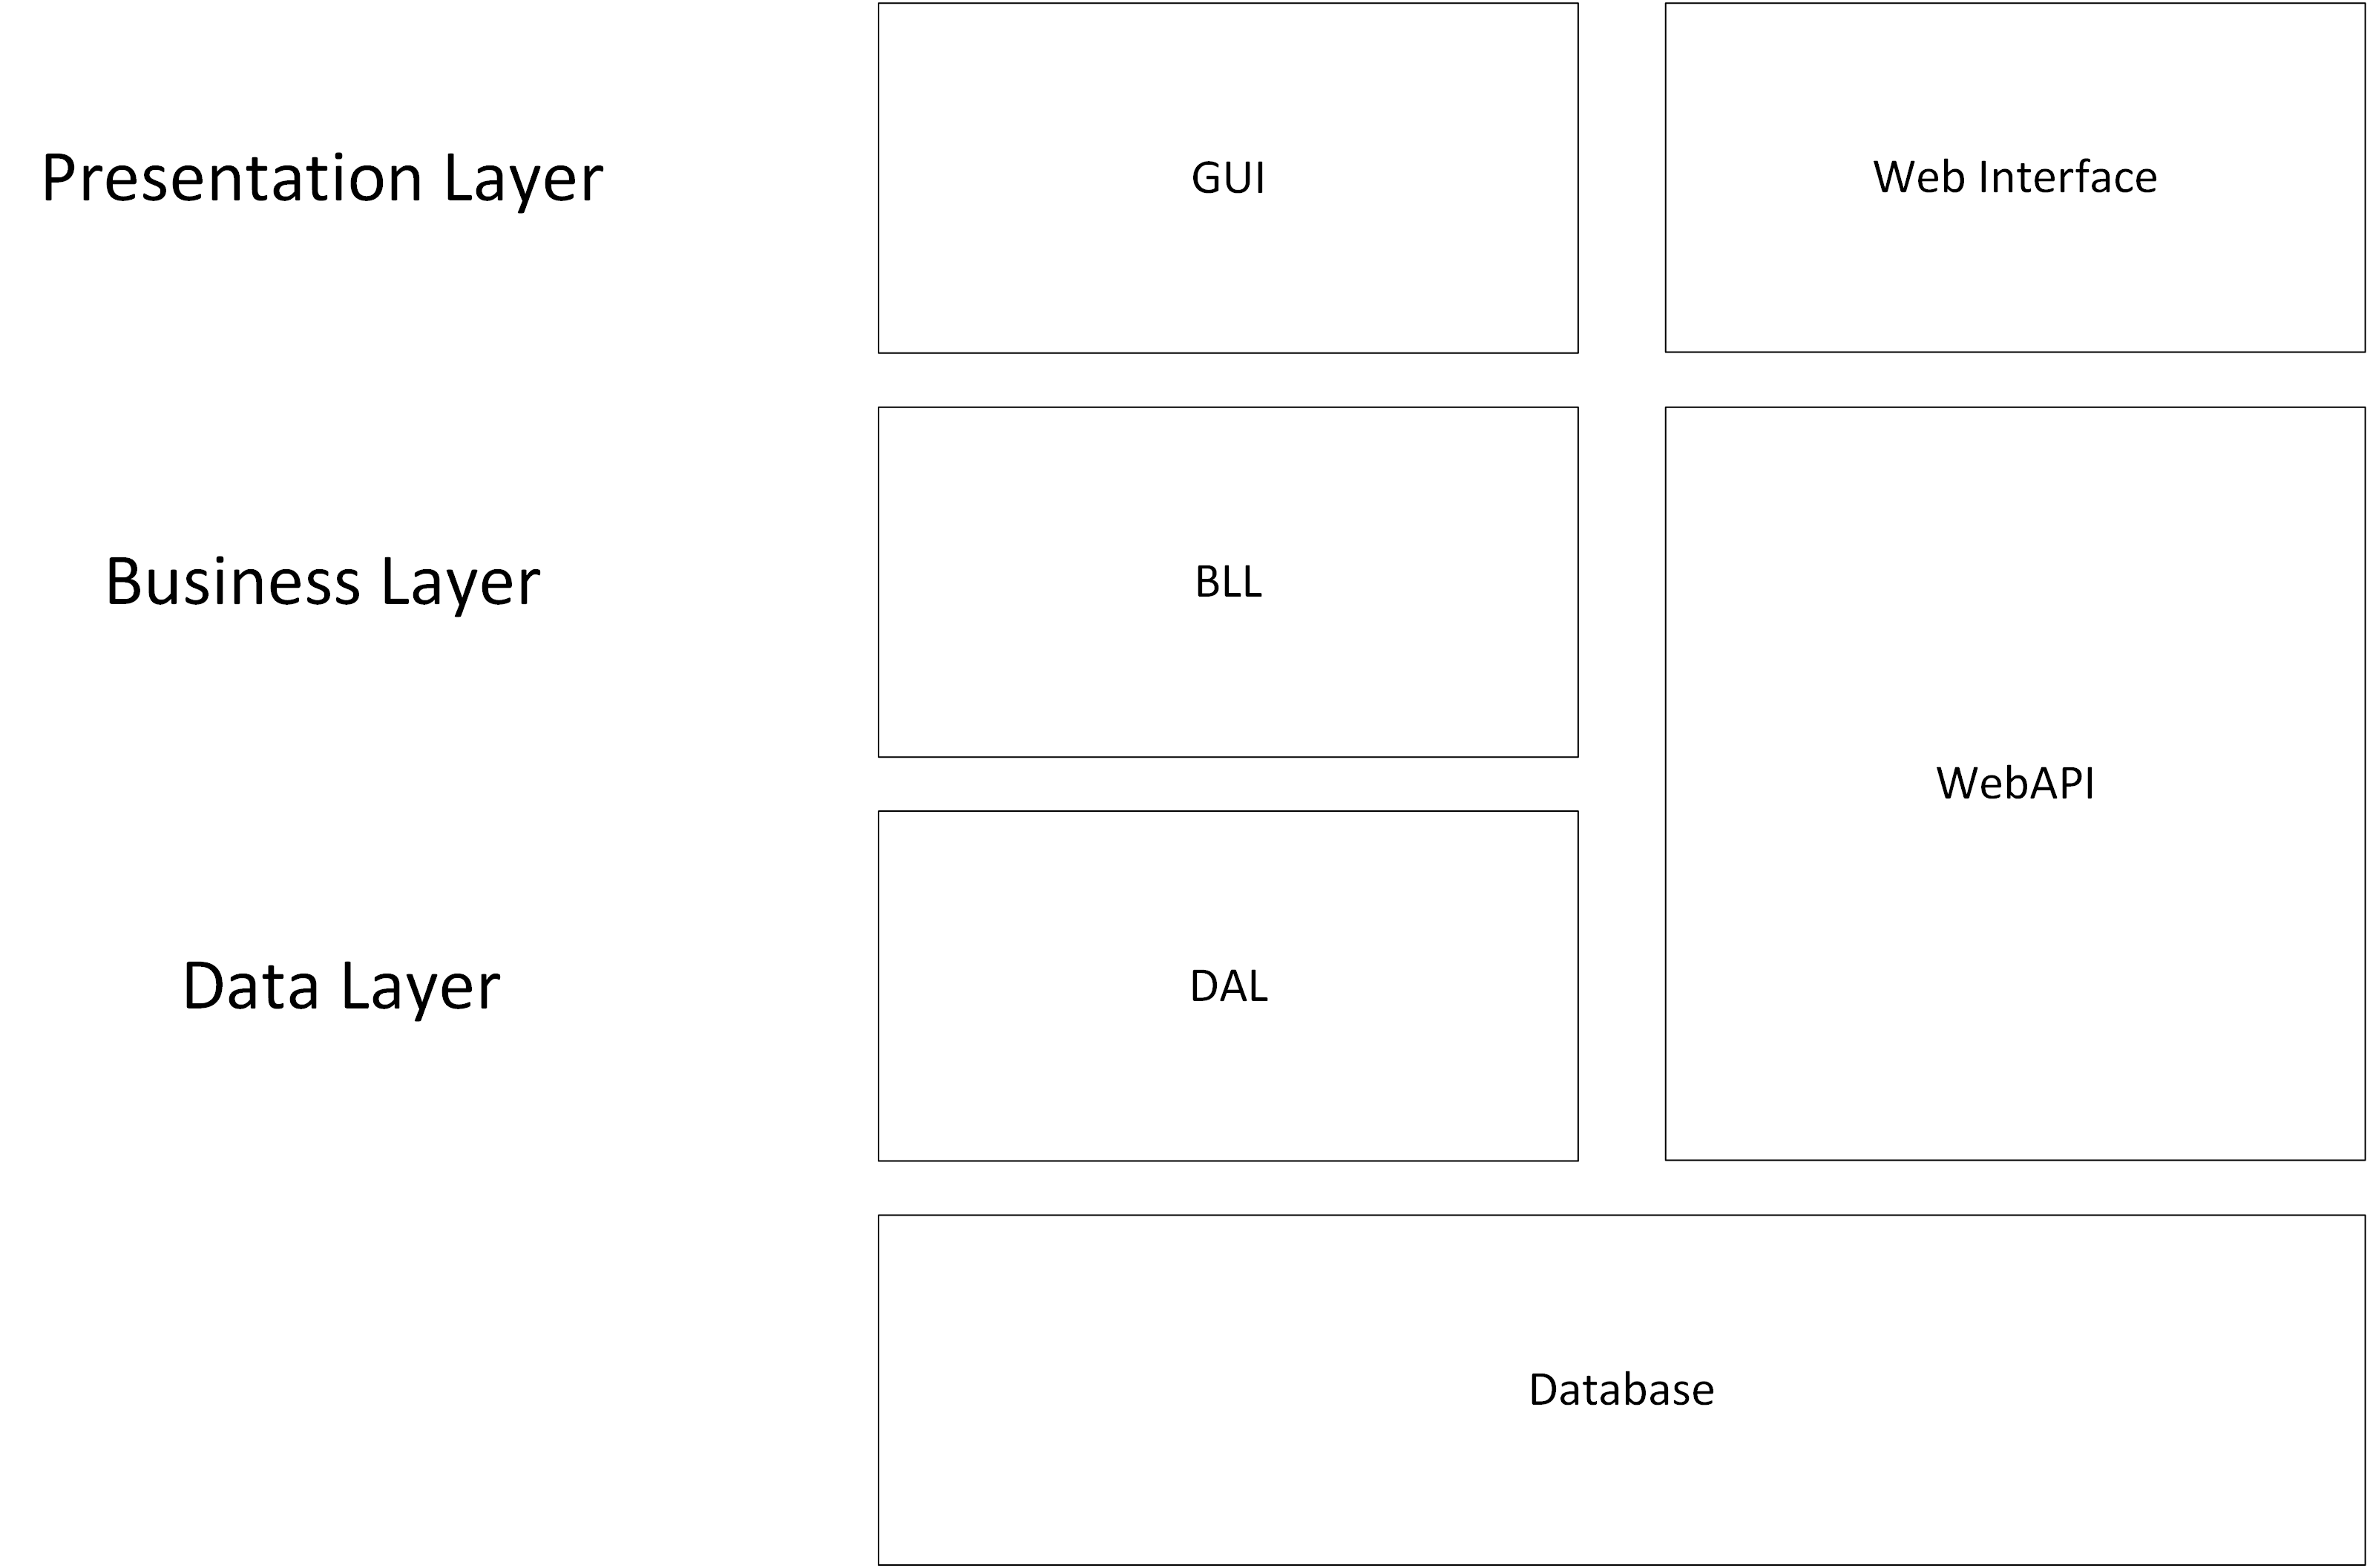
\includegraphics[width=0.75\textwidth]{Rapport/3tier}
	\caption{Overordnet system}
	\label{ArkiDia}
\end{figure}

\subsection{N+1 view}
Arkitekturen er beskrevet med N+1, som er en specialisering af 4+1, der beskrevet i artiklen af \cite{4plus1}. Specialiseringen gør det muligt at tilføje og fjerne de Views, som giver eller ikke giver mening for beskrivelsen af \gls{system}et.

\subsubsection{Use Case View}
I Use Case Viewet kan der ses hvordan de forskellige \gls{usecase}s beskriver systemet. Der er i dokumentationen indsat overordnede diagrammer, der beskriver handlingsforløbet for hver af de fully dressed \gls{usecase}s.

\subsubsection{Logical View}
Logical View er en oversigt over, hvordan programmet er bygget op. Logical View viser her, hvordan det er valgt at dele systemet op i lag for at give mere overskuelighed. Her er der tale om:
\begin{itemize}
	\item Presentation Layer
	\item Business Layer
	\item Data Layer
	\item Web API
\end{itemize}
 
\textbf{Presentation Layer} indeholder alt omkring \gls{GUI} og hvordan den er bygget op ved hjælp af \gls{MVVM}. Her introduceres de forskellige \gls{Views}: SalesView, NumpadView, TabView, SettingsView. Disse bliver alle modelleret af en tilhørende \gls{ViewModel} således at de forskellige \gls{Views} intet kendskab har til Business Layer. \textbf{Business Layer} indeholder alt omkring oprettelse af ordrer og transaktioner. Dette lag kommunikerer med Presentation Layer og ligeledes med Data Layer. Det er Business Layer der sørger for at hente gemte data i Data Layer og ligeledes give data til Presentation Layer.\newline
\textbf{Data Layer} står for al persistering af data. Her bliver data gemt i en database og ligeledes hentet derfra. Data kan kun blive tilgået via \gls{DAL}.\newline
\textbf{WebAPI} sørger for at det er muligt at oprette, redigere og fjerne produkter fra databasen. Her er det også muligt at få vist statistik over igangværende og forhenværende salg i systemet. 

\subsubsection{Deployment View}
I Deployment View ses der hvordan systemet kunne udrulles og sættes op. Her er det vigtig at bide mærke i at selve databasen og \gls{WebAPI}'et kunne sættes op på deres egne seperate computere fungerende som server, og GUI'en og business logikken, kunne køre på en anden computer som så kunne kobles op til serveren. I vores system som det er udviklet, ligger databasen på samme computer som resten af systemet. \newline\newline
\begin{figure}[H]
	\centering
	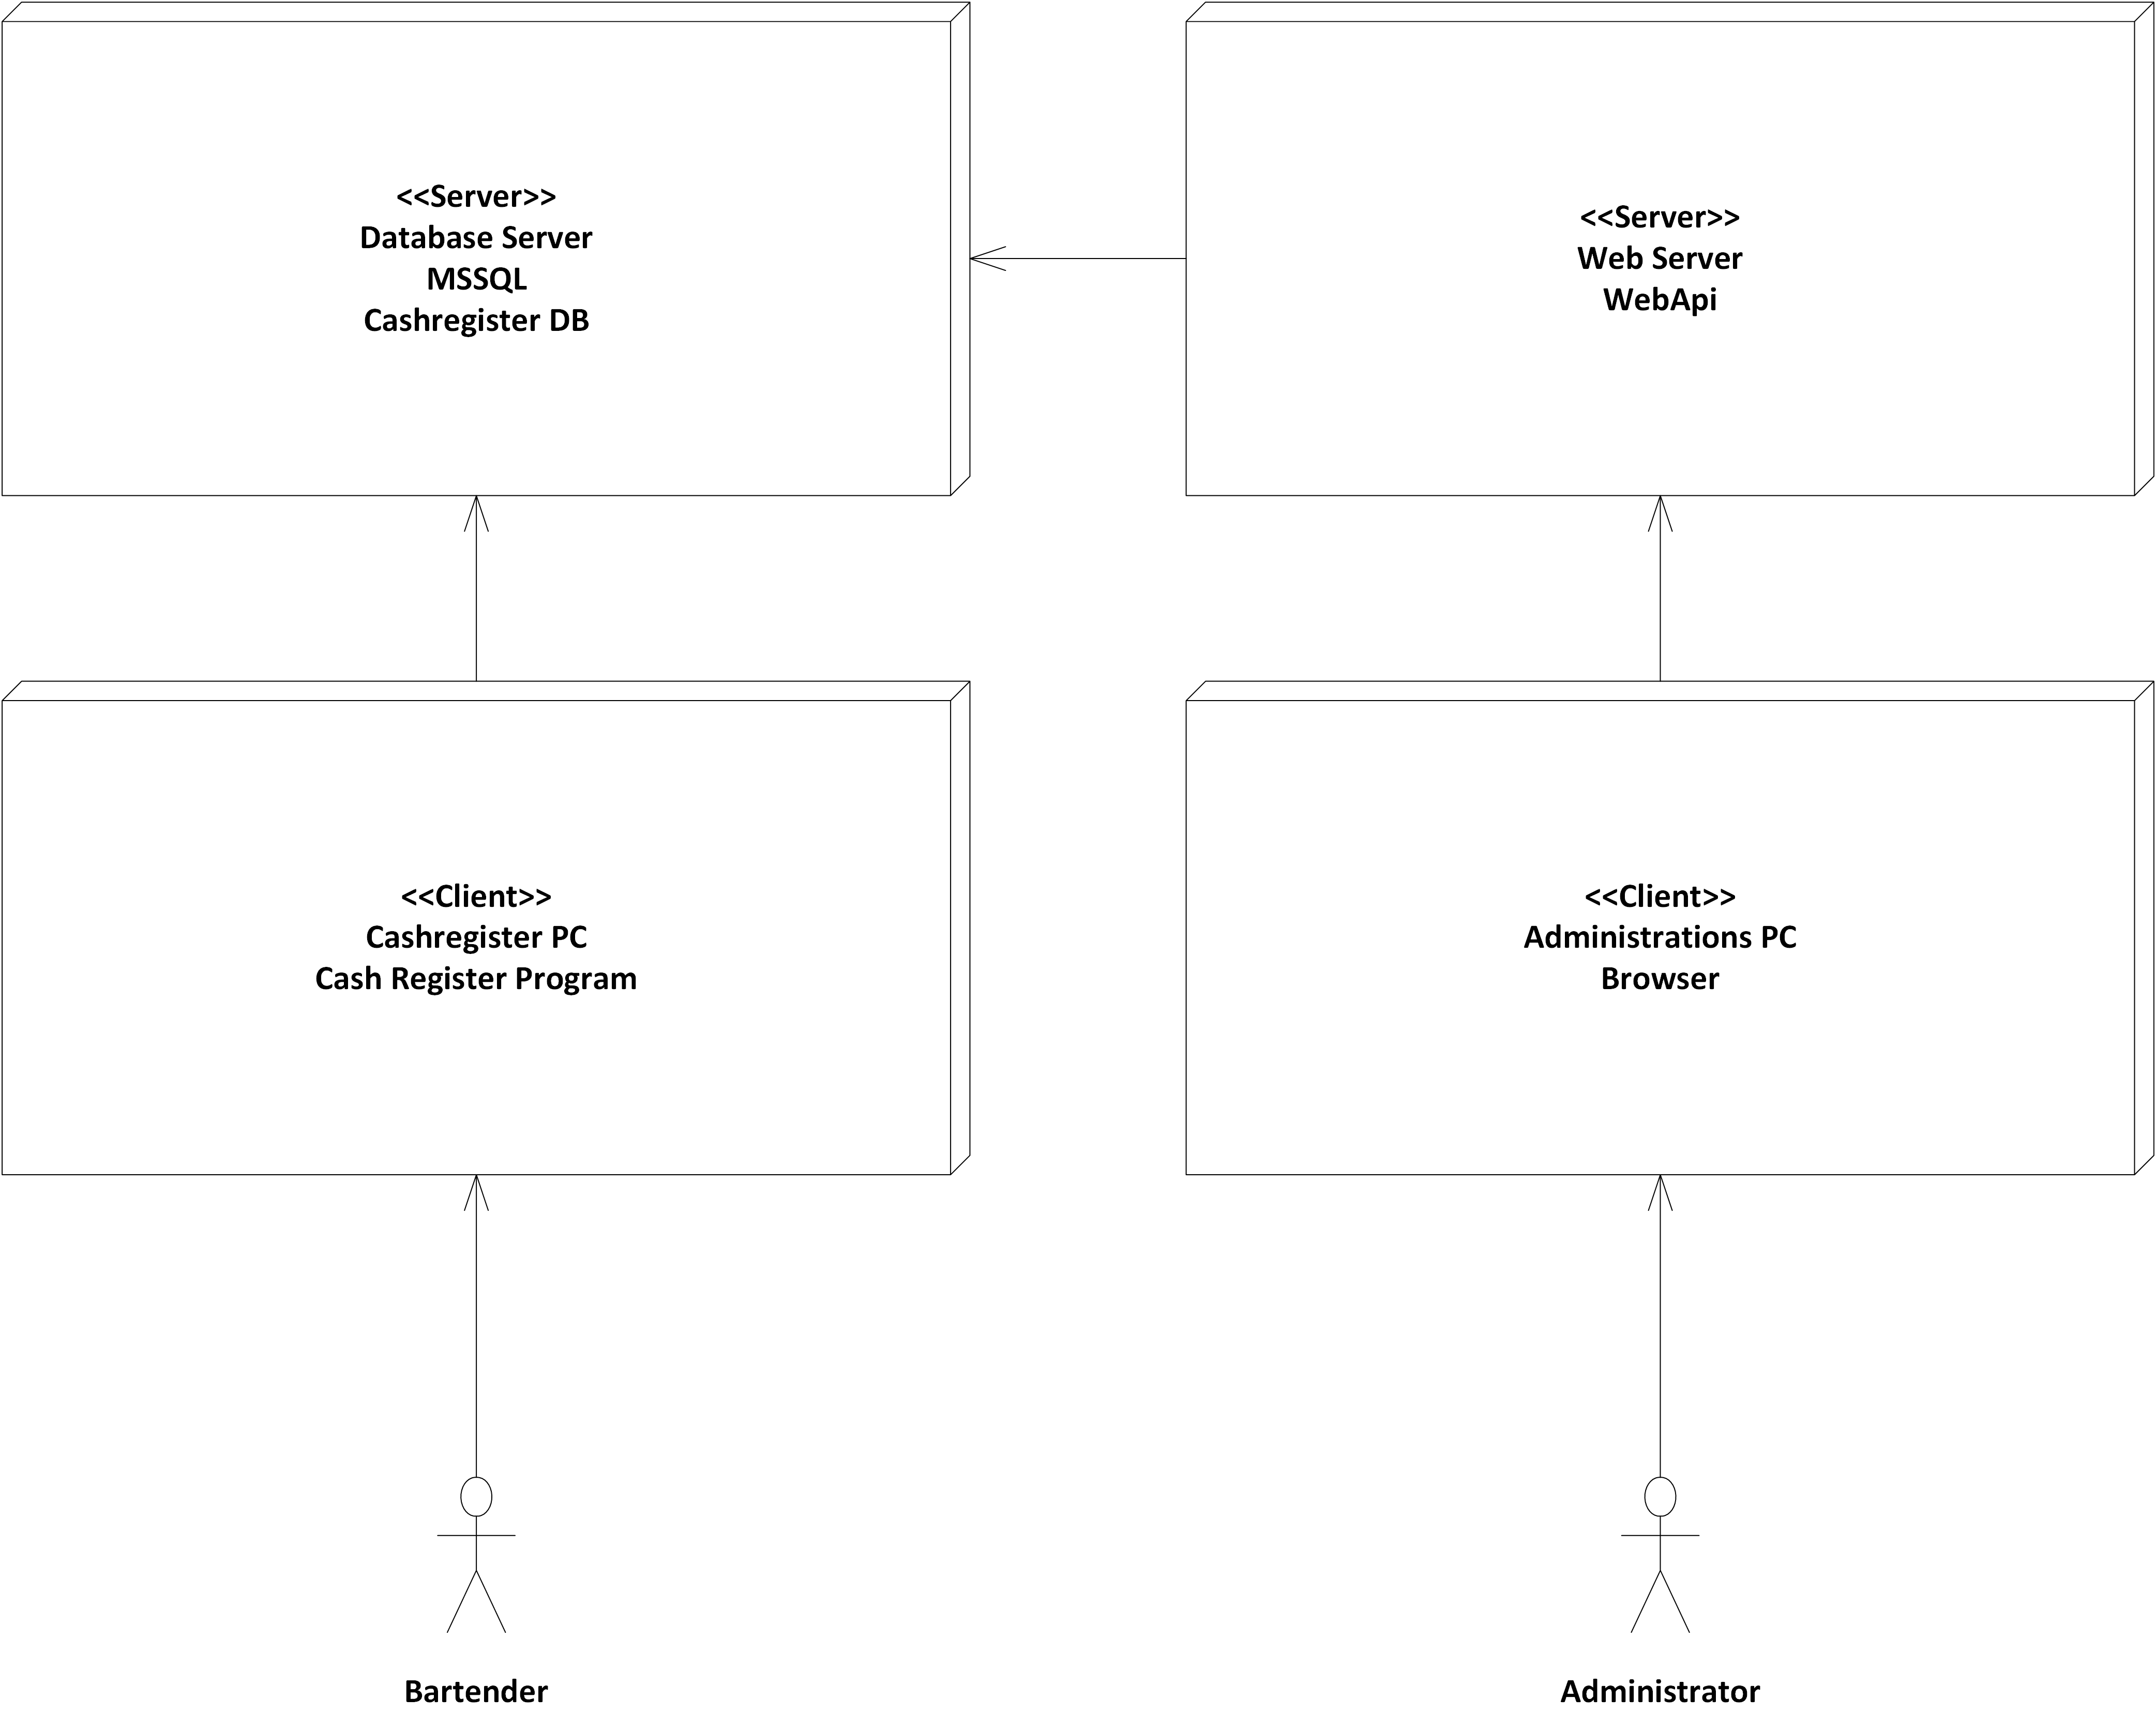
\includegraphics[scale=0.6]{/N+1/DeploymentView/System/Diagrammer/DEPLOY}
	\caption{Diagram over deployment af system}
	\label{fig:DeplayDia}
\end{figure}
Som det ses af figur \ref{fig:DeplayDia} kunne man sætte en administrations PC op som ville koble op til en Web Server som ville hoste Web API'et. Web API'et ville så tilkoble sig Database serveren so  ville køre på en seperat server. Hertil ville CashRegister programmet så køre på en seperat PC som bartenderen ville have adgang til. Dette betyder at man kunne opsætte flere kasseapparater som kunne koble op til samme database.  

\subsubsection{Data View}
I Data View beskrives overgangen fra objekter i systemet til databasen. Her bliver en Mapping til databasen.\newline\newline
I dokumentationen er der beskrevet hvor de forskellige klasser er blevet mappet til databasen. Her bliver der gennemgået hvorfor tabellerne er sat op som de er, og hvordan deres forhold til hinanden er. Her er klasse modeller og de fysiske modeller sat op over for hinanden så man hurtig kan se forskelle og ligheder.

\begin{figure}[H]
	\centering
	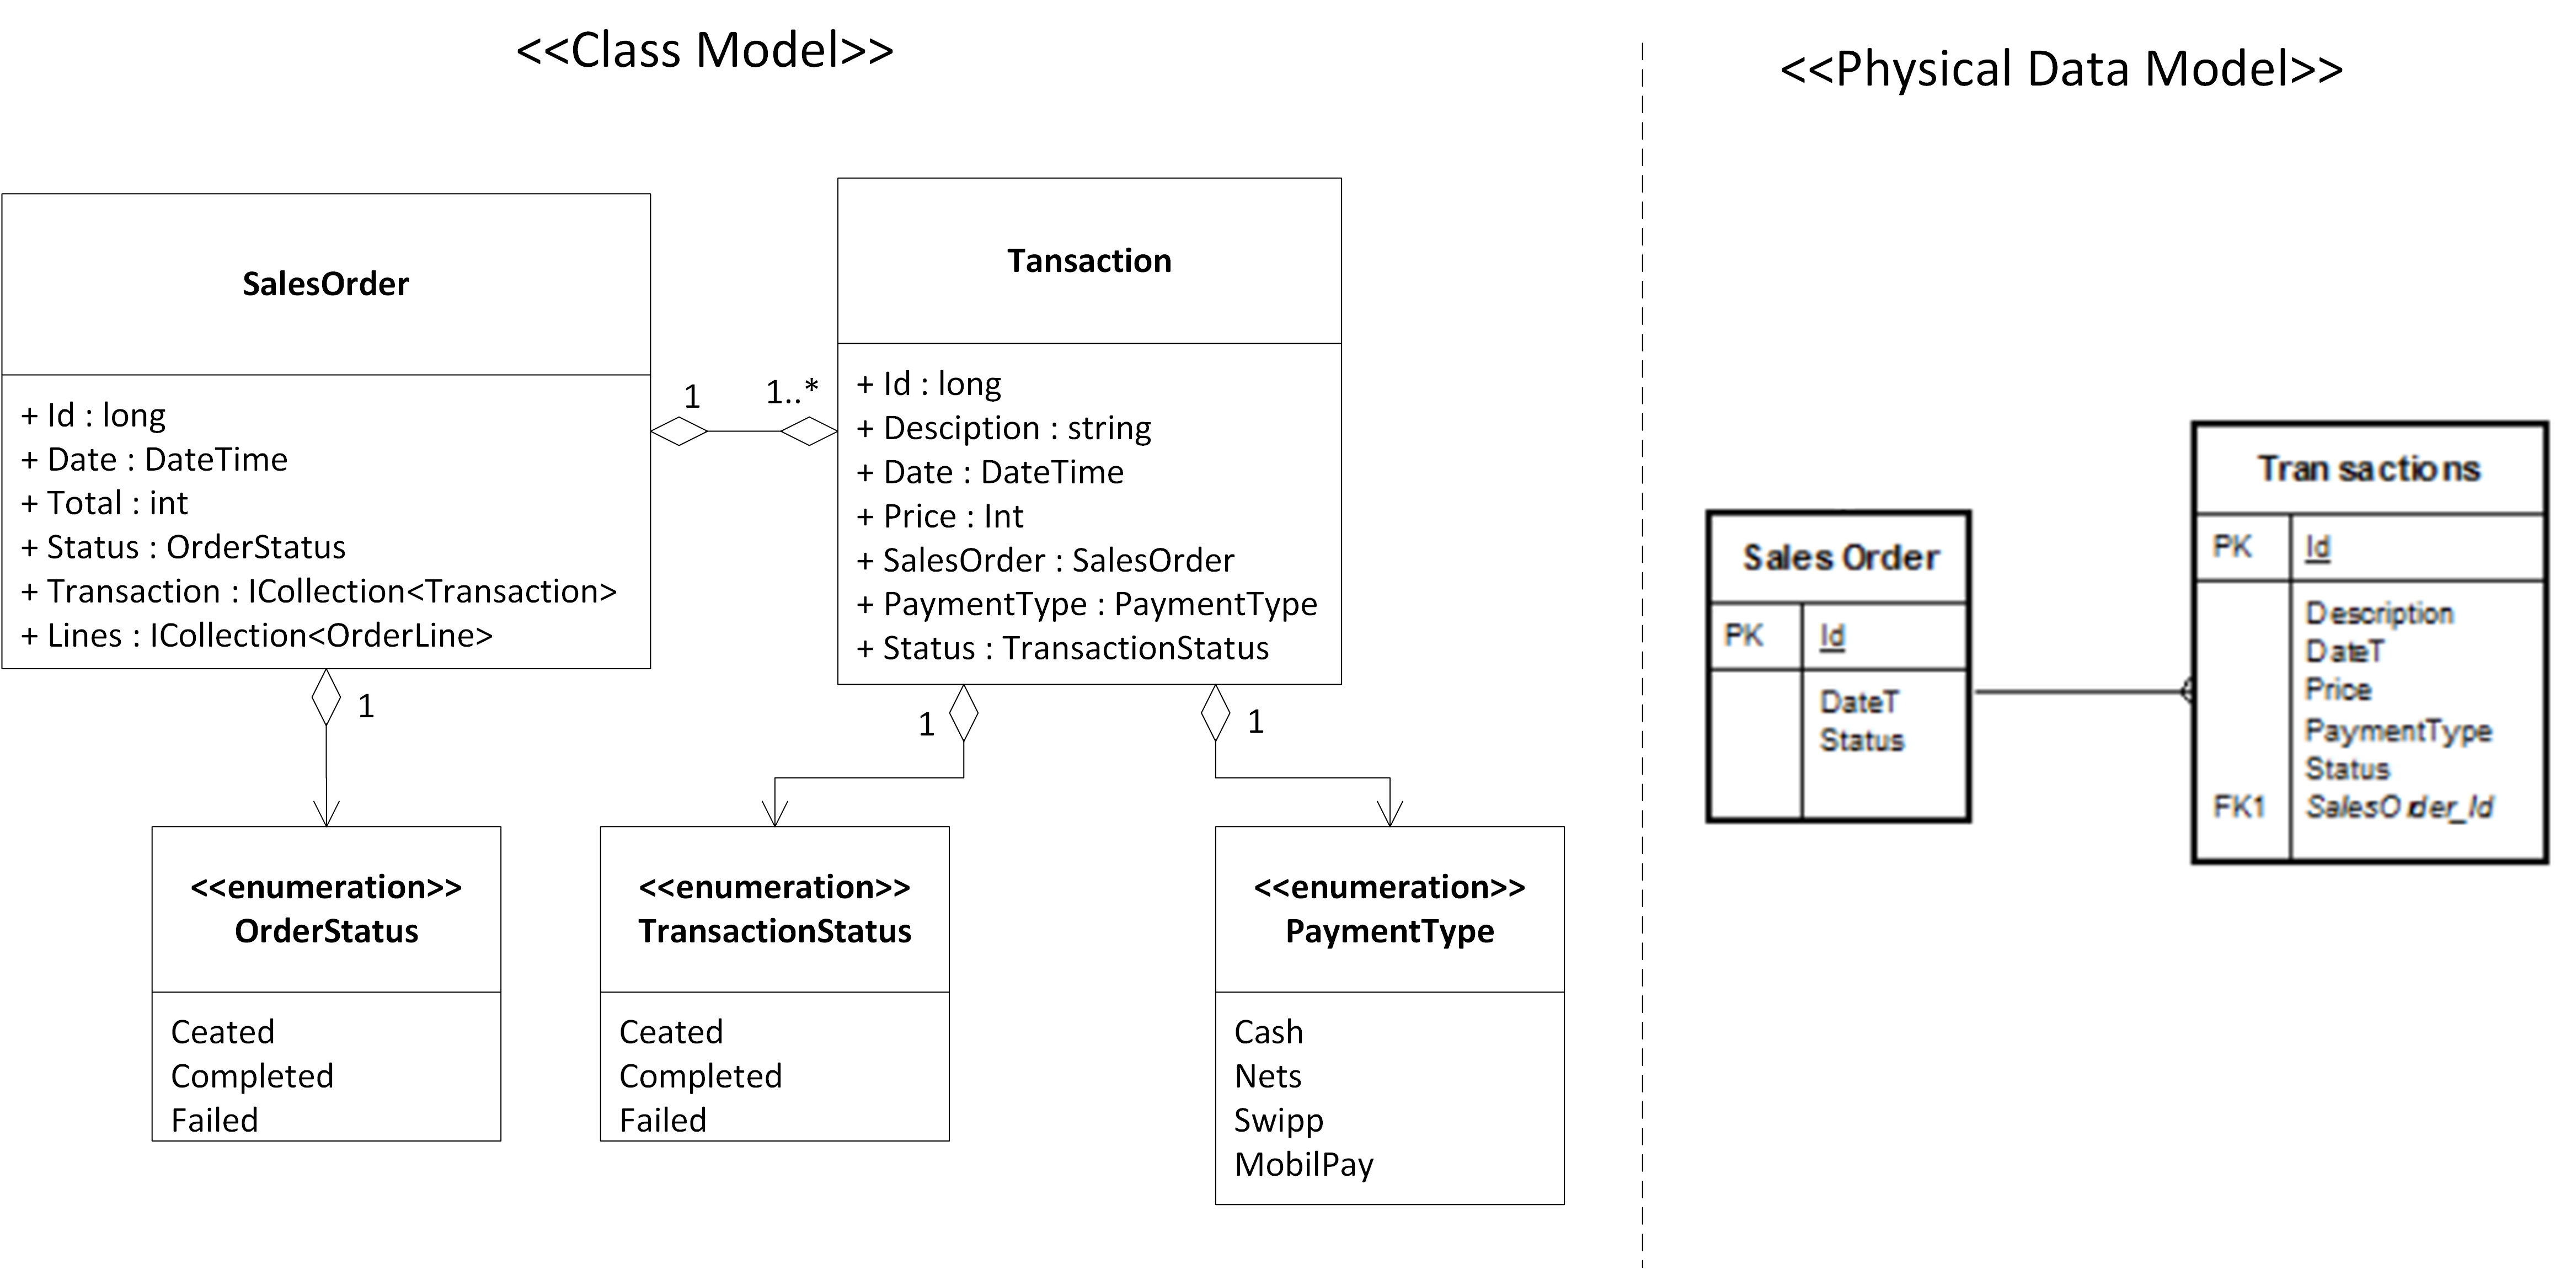
\includegraphics[scale=0.6]{/N+1/DataView/mapping/Mapping1}
	\caption{Diagram over objekt mapping}
	\label{MapDia}
\end{figure}	

På figur \ref{MapDia} ses det hvordan kobling af SalesOrder sker til Databasen. Her kan det ses at der mellem SalesOrder og Transaction er et one-to-many forhold og at Transaction har en fremmednøgle til SalesOrder.\newline\newline
Ydermere kan der i Data View ses hvordan dataflows sker fra én handling til den næste sker. Hertil er der lavet nogle aktivitetsdiagrammer ud fra de definerede Use Cases. 

\begin{figure}[H]
	\centering
	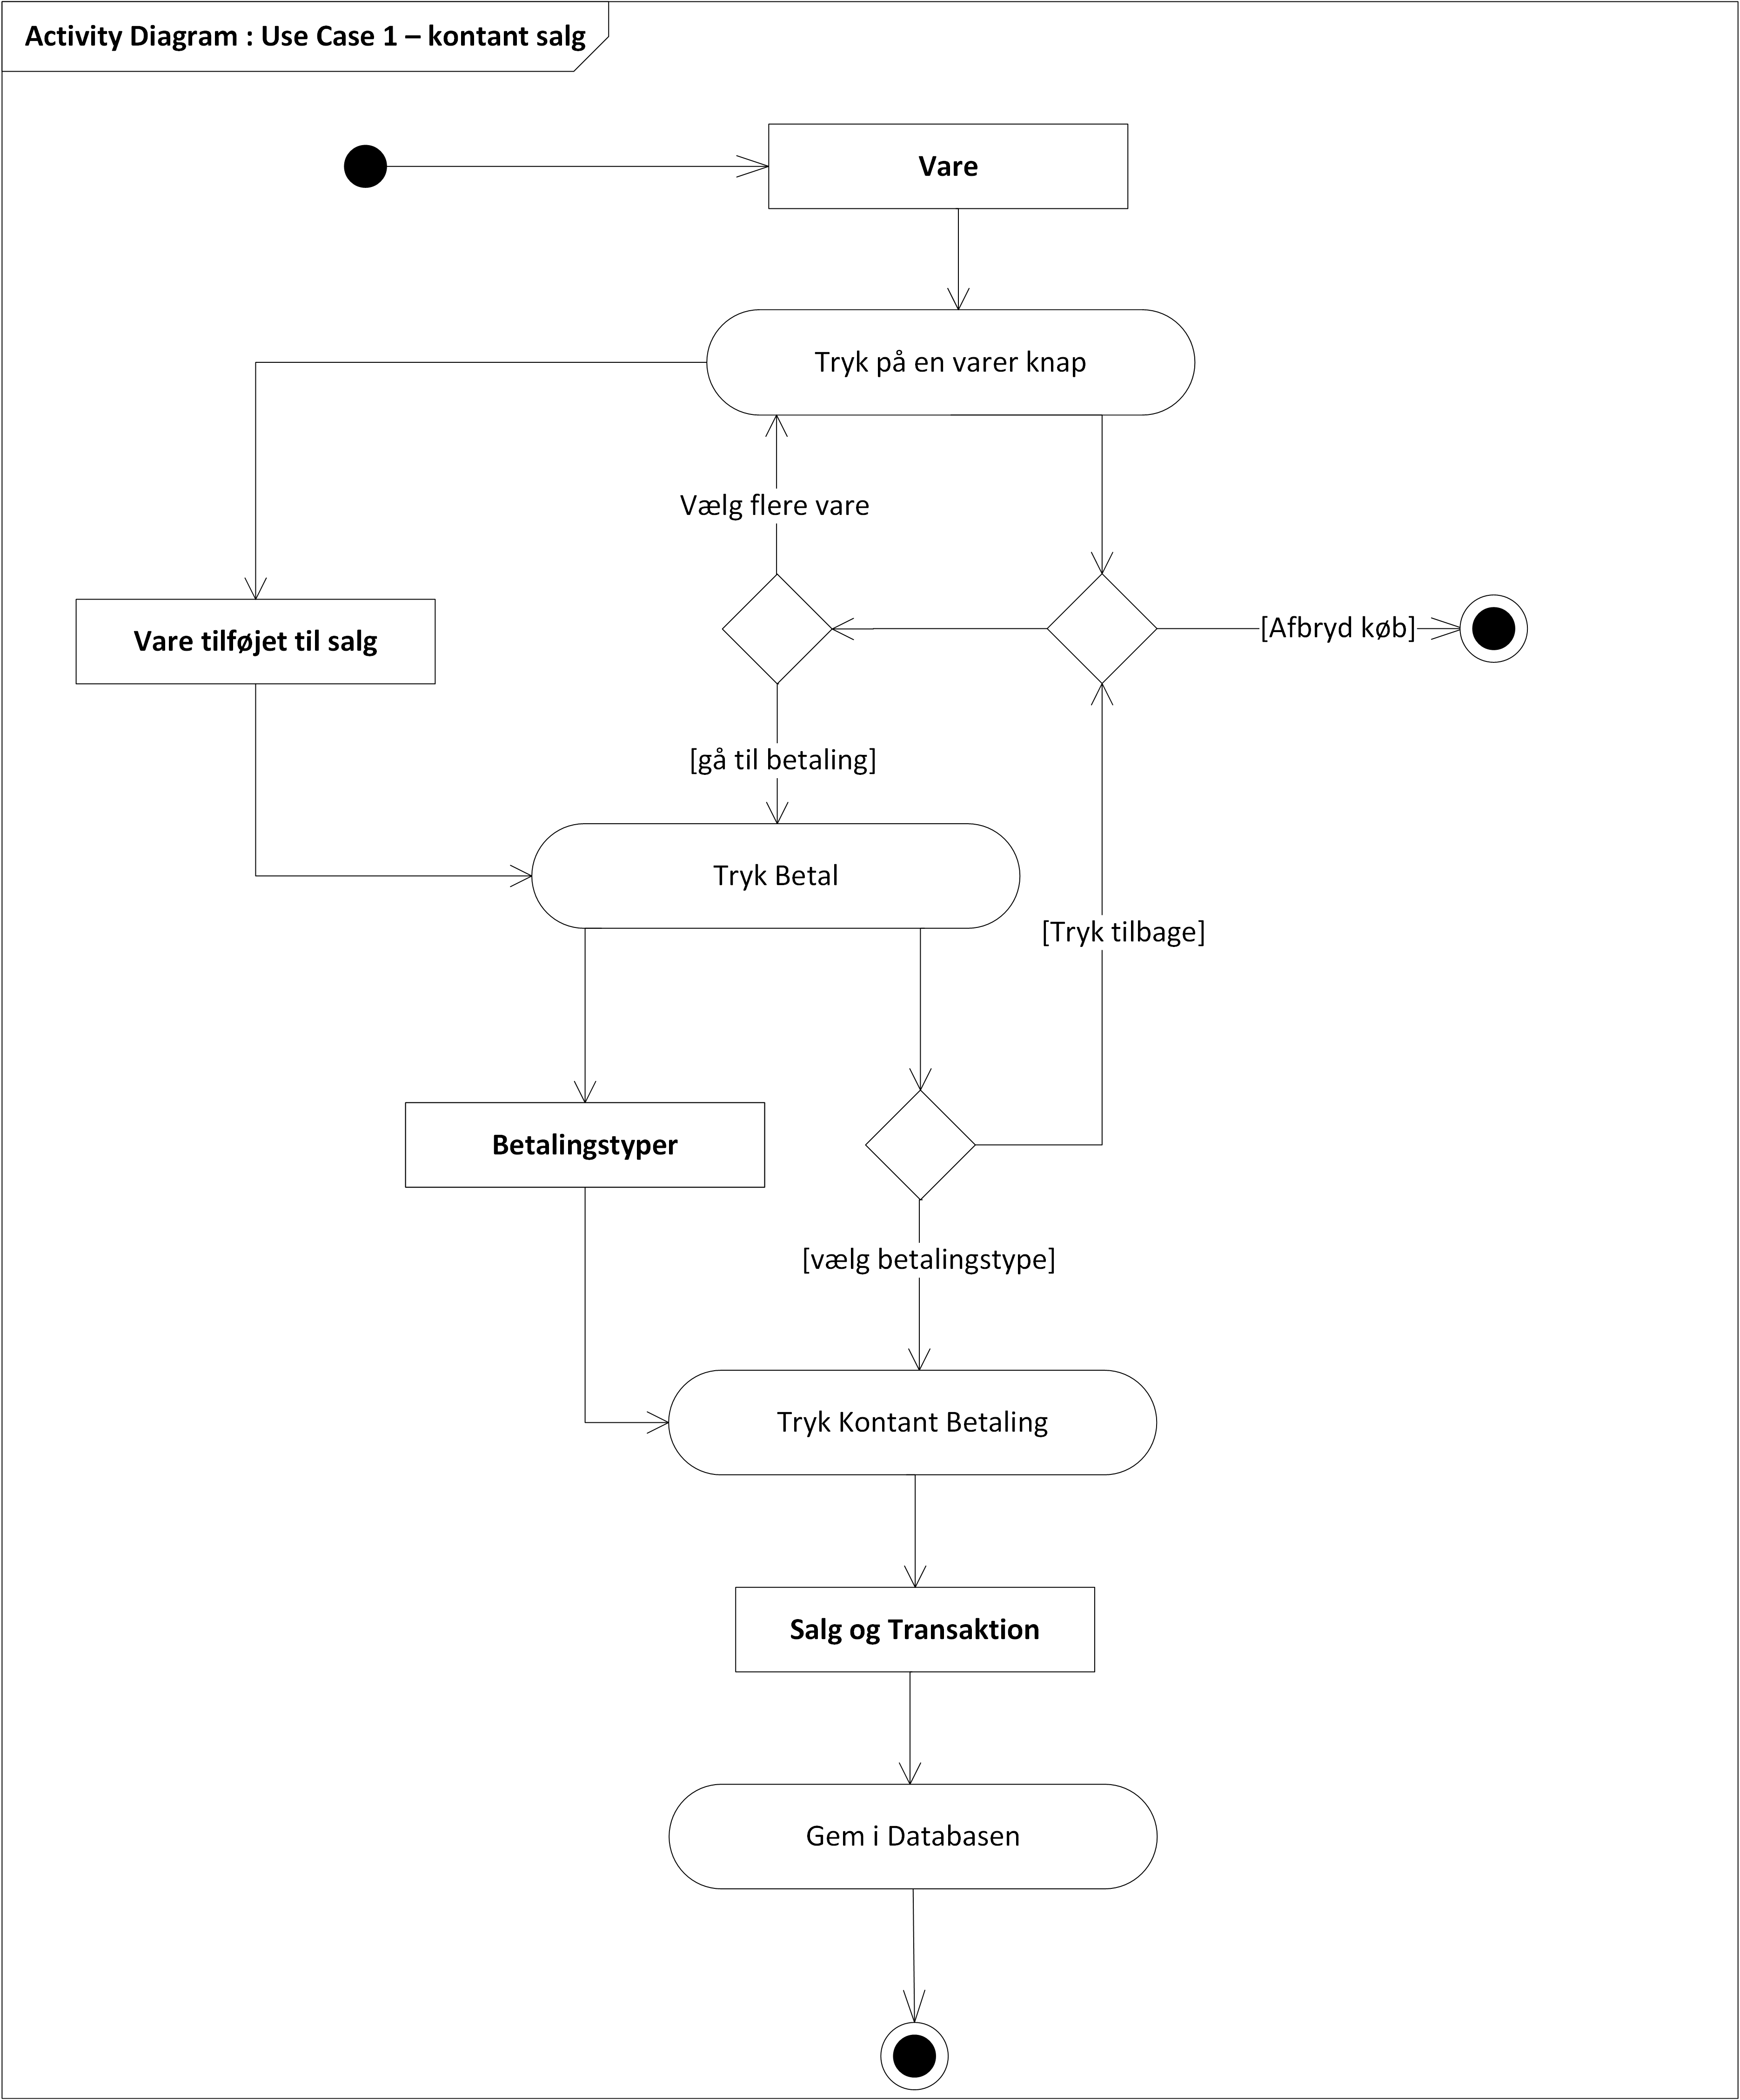
\includegraphics[scale=0.6]{/N+1/DataView/DataFlow/UC1}
	\caption{Aktivitetsdiagram over Use Case 1}	
	\label{AktDia}
\end{figure}

På figur \ref{AktDia} er dataflowet i forhold til Use Case 1 illustreret via et aktivitetsdiagram. Aktiviteterne gentages i nogle tilfælde og kører derfor i en løkke, og det kan også ses hvornår Use Casen og hvordan Use Casen afsluttes. Alt dette står mere detaljeret beskrevet i dokumentationen. 

 
 
  

